\chapter{Introduzione}

\section{Prima Lezione}
Un Sistema Operativo (SO) agisce come intermediario tra l'utente e l'hardware, fornendo gli strumenti per un uso corretto delle risorse della macchina (CPU, memoria, periferiche). Ha due obiettivi principali:
\begin{itemize}
    \item Dal punto di vista dell'utente: rendere il sistema facile da usare.
    \item Dal punto di vista della macchina: ottimizzare l'uso delle risorse in modo sicuro ed efficiente.
\end{itemize}

\subsection{Architetture Single/Multi-Core}
Negli anni 2000 si è passati da processori single-core a multi-core, con CPU dotate di più core in grado di eseguire istruzioni di programmi diversi simultaneamente.

\subsection{Tipi di Eventi}
\begin{itemize}
    \item \textbf{Interrupt}: Eventi di natura hardware, rappresentati da segnali elettrici inviati da componenti del sistema.
    \item \textbf{Eccezioni}: Eventi di natura software, causati dal programma in esecuzione. Le eccezioni si dividono in:
    \begin{itemize}
        \item \textit{Trap}: Causate da malfunzionamenti del programma (es. accesso a memoria non autorizzato, divisione per 0).
        \item \textit{System Call}: Richiesta di servizi al SO, come l'accesso ai file.
    \end{itemize}
\end{itemize}

\subsection{Gestione degli Eventi}
Quando si verifica un evento:
\begin{enumerate}
    \item \textbf{Salvataggio dello stato della CPU}: Il Program Counter (PC) e i registri della CPU vengono salvati in appositi registri speciali per poter riprendere l'esecuzione successivamente.
    \item \textbf{Esecuzione del codice del SO}: Il \textbf{PC} viene aggiornato con l'indirizzo del codice del \textbf{SO} che gestisce l'evento, memorizzato in una tabella detta \textit{vettore delle interruzioni}. Questo vettore contiene puntatori a differenti routine di gestione eventi.
    \item \textbf{Return}: Una volta gestito l'evento, il SO ripristina lo stato precedente e l'esecuzione del programma sospeso riprende.
\end{enumerate}
\nt{
    Nel Program Counter viene scritto l'indirizzo in RAM della porzione di codice del So che serve a gestire l'evento che si è appena verificato.
    All'accensione del computer, il SO stesso carica in aree della RAM che il SO riserva a se stesso le varie porzione di codice eseguibile che dovranno entrare in esecuzione quando si verifica un eccezione.
}
\clm{}{}{
    Nei primi N indirizzi della RAM viene caricato una array di puntatori noto come \textbf{vettore delle interruzioni}. Ogni entry del vettore contiene l'indirizzo di partenza in RAM di una delle porzioni di codice del SO del punto precedente.
}
Quando un certo vento si verifica, il program counter viene aggiornato con il valore che è indicato nella cella di memoria collegata all'entry point dell'eccezione.
L'ultima istruzione di ogni procedura di gestione di un evento sarà sempre una istruzione di "return from event" (\textbf{ra}).



\section{Struttura della Memoria}
Nel contesto del \textbf{SO}, ci sono due principali tipi di memoria:
\begin{itemize}
    \item \textbf{Memoria Principale} (\textit{RAM}): Memoria primaria in cui risiedono programmi e dati durante l'esecuzione.
    \item \textbf{Memoria Secondaria}: Memoria di massa, come \textbf{hard disk} o \textbf{memorie a stato solido}, utilizzata per la conservazione permanente dei dati.
\end{itemize}

\section{Gerarchia delle Memorie}
\textbf{Nella figura}: \textit{Velocità implica complessità maggiore, costo maggiore e capacità minore.}
\begin{itemize}
    \item \textbf{Caching}: Ogni livello di memoria fa da cache per il livello successivo. Esempio: la \textbf{RAM} fa da cache per l'\textbf{hard disk}, la \textbf{CACHE} per la \textbf{RAM}, e i \textbf{registri della CPU} per la \textbf{CACHE}.
\end{itemize}

\begin{figure}[ht!]
    \centering
    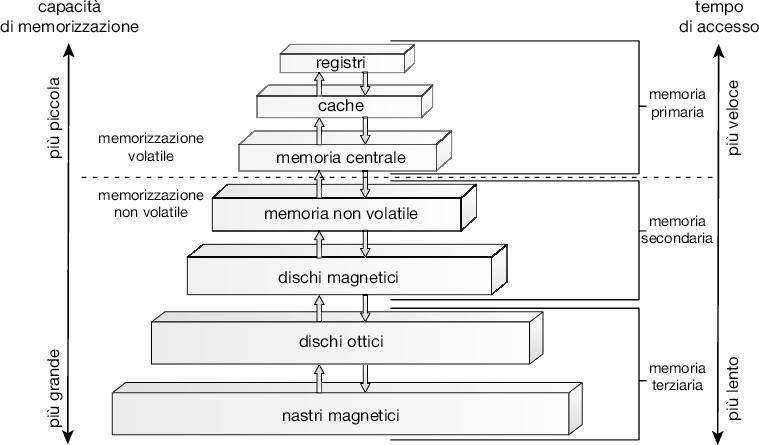
\includegraphics[width=10cm]{images/gerarchia delle memorie.png}
    \label{fig:gerarchy-of-memory}
\end{figure}

\qs{}{
Sarebbe bello avere 500GB di registri di CPU o Hard Disk veloci quando i registi della CPU?
}
Per una informazione  la si deve copiare in una memoria più veloce (più costosa).
La \textbf{RAM} fa da cache per l'HDD.
La \textbf{CACHE} fa da cache per la RAM
I \textbf{REGISTRI} fanno da cache per la CACHE.

\subsubsection{Due tecnlogie di memoria RAM}
\begin{itemize}
    \item SRAM: per la cache e i registri della CPU
    \begin{itemize}
        \item Creato con i FLIP-FLOP, questo porta un costo maggiore ma una maggiora efficienza rispetto alla DRAM.
    \end{itemize}
    \item DRAM: per la memoria principale/centrale
    \begin{itemize}
        \item Creato con i Condensatori, che tendono a perdere il loro stato. Questo obbliga a refresharli costantemente portando un dispendio maggiore di energie ma un minore costo di produzione.
    \end{itemize}
\end{itemize}

\section{Struttura di I/O}
Un generico computer è composto da una CPU e da un insieme di dispositivi di I/O connessi fra loro da un bus comune.
Ogni dispositivo di I/O è controllato da un apposito componente hardware detto \textbf{controller}
Il controller è a sua volta un piccolo processore, con alcuni registri e una memoria interna, detto \textbf{buffer}.
il SO interagisce con il controller attraverso un software apposito noto come \textbf{driver del dispositivo}.
\ex{Driver}{
Il driver del dispositivo, carica nei registri dei controller opportuni valori che specificano le operazioni da compiere.\\
Il controller esamina i registri e intraprende l'operazione corrispondente.\\
Il controller trasferisce i dati dal dispositivo al proprio buffer.\\
Il controller invia un interrupt al SO indicando che i dati sono pronti per essere prelevati. \\
}

Questo modo di gestire l'IO con grandi quantità di dati è molto \textbf{inefficiente}.
Una soluzione utile è avere un canale di comunicazione diretto tra il dispositivo e la RAm, in modo da non "disturbare" troppo il SO.
Tale canale è detto \textbf{Direct Memory Access} (DMA).
Il SO, tramite il driver del disco, istruisce opportunamente il controller del disco, con un comando (scritto nei registri del controller) del tipo:
\clm{}{}{Trasferisci il blocco numero 1000 del disco in RAM a partire dalla locazione di RAM di indirizzo F2AF}
Il controller trasferisce direttamente il blocco in RAM usando il DMA, e ad operazione conclusa avverte il SO mediante un interrupt opportuno.


\section{Multitasking e Time-Sharing}
Quando lanciamo un programma, il SO cerca il codice del programma sull’hard disk, lo copia in RAM, e \textit{"fa partire il programma"}
Noi utenti del SO non dobbiamo preoccuparci di sapere dov’è memorizzato il programma sull’hard disk, né dove verrà caricato in RAM per poter essere eseguito.

Dunque, il SO rende \textbf{facile} l’uso del computer. Ma il SO ha anche il compito di assicurare un uso \textbf{efficiente} delle risorse del computer, in primo luogo la CPU stessa.

\clm{}{}{
Consideriamo un programma in esecuzione: a volte deve fermarsi temporaneamente per compiere una operazione di I/O (esempio: leggere dall’hard disk dei dati da elaborare). \\
Fino a che l’operazione non è completata, il programma non può proseguire la computazione, e non usa la CPU.\\
Invece di lasciare la CPU inattiva, perché non usarla per far eseguire il codice di un altro.
}
Questo è il principio della multiprogrammazione (multitasking), implementato da tutti i moderni SO: il SO mantiene in memoria principale il codice e i dati di più programmi che devono essere eseguiti. (Detti anche job)
\begin{figure}[h]
    \centering
    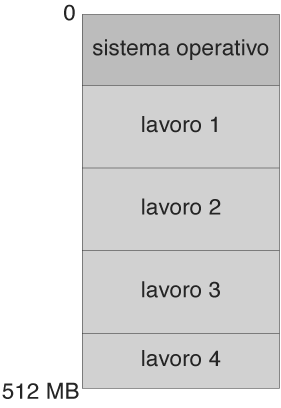
\includegraphics[width=0.25\linewidth]{images/multiprogramming-stack.png}
\end{figure}

\qs{}{Alcune applicazioni degli utenti però sono per loro natura interattive, come fa ad esserci una interazione continua tra il programma e l'utente che lo usa?}
Oltre a questo, i sistemi di calcolo son multi-utente cioè permettono di essere connessi al sistema e di usare "contemporaneamente" il sistema stesso.

\subsection{Time-Sharing}
È meglio allora \textbf{distribuire} il tempo di CPU fra i diversi utenti (i loro programmi in "esecuzione") frequentemente (ad esempio ogni 1/10 di secondo) così da dare una impressione di \textbf{simultaneità} (che però è solo apparente).

Questo è il \textbf{time-sharing}, che estende il concetto di \textbf{multiprogrammazione}, ed è implementato in tutti i moderni sistemi operativi.

\section{Compiti del sistema operativo}

E’ necessario tenere traccia di tutti i programmi \textbf{attivi} nel sistema, che stanno usando o vogliono usare la CPU, e gestire in modo appropriato il passaggio della CPU da un programma all’altro, nonché \textbf{lanciare} nuovi programmi e \textbf{gestire} la terminazione dei vecchi.
\nt{Questo è il problema della gestione dei processi (cap. 3) e dei thread (cap. 4)}.

Quando la CPU è libera, e più programmi voglionousare, a quale programma in RAM assegnare la CPU?
\nt{Questo è il problema di CPU Scheduling (cap. 5)}

I programmi in esecuzione devono interagire fra loro senza danneggiarsi ed evitando situazioni di stallo (ad esempio, il programma A aspetta un dato da B che aspetta un dato da C che aspetta un dato da A)
\nt{Questi sono i problemi di sincronizzazione (cap. 6/7) e di deadlock (stallo dei processi) (cap. 8)}

Come gestire la RAM, in modo da poterci far stare tutti i programmi che devono essere eseguiti? Come tenere traccia di quali aree di memoria sono usate da quali programmi?
\nt{La soluzione a questi problemi passa attraverso i concetti di gestione della memoria centrare (cap. 9) e di memoria virtuale (cap. 10).}

Infine, un generico computer è spesso soprattutto un luogo dove gli utenti \textbf{memorizzano} permanentemente, organizzano e recuperano vari tipi di informazioni, all’interno di "contenitori" detti \textbf{file}, a loro volta suddivisi in cartelle (o folder, o directory) che sono organizzate in una struttura gerarchica a forma di albero (o grafo aciclico) nota come \textbf{File System}.

\nt{Il SO deve gestire in modo efficiente e sicuro le informazioni memorizzate nella memoria di massa (o secondaria) (cap. 11) deve permettere di organizzare i propri file in modo efficiente, ossia fornire una adeguata interfaccia col file system (cap. 13), deve implementare il file system (cap. 14)}

\qs{}{come fa il SO a mantenere sempre il controllo della macchina?}
Soprattutto, come fa anche quando non sta girando?
Ad esempio, come evitare che un programma utente acceda direttamente ad un dispositivo di I/O usandolo in maniera impropria?
Oppure, che succede se un programma, entra in un loop infinito?
E’ necessario prevedere dei modi per proteggersi dai malfunzionamenti dei programmi utente (voluti, e non)

\subsection{Duplice modalità di funzionamento}

Nei moderni processori le istruzioni macchina possono
essere eseguite in due modalità diverse:
\begin{enumerate}
    \item normale (modalità utente)
    \item di sistema (modalità priviligiata, o kernel / monitor / supervisor mode)
\end{enumerate}
La CPU è dotata di un “bit di modalità” di sistema (0) o utente (1), che permette di stabilire se l’istruzione corrente è in esecuzione per conto del SO o di un utente normale.

\clm{}{}{
Le istruzione macchina \textbf{sensibili}, nel senso che se usate male possono danneggiare il funzionamento del sistema nel suo complesso, possono essere eseguite solo in modalità di sistema, e quindi solo dal SO, altrimenti se nel codice di un programma normale in esecuzione è contenuta una istruzione delicata, quando questa istruzione entra nella CPU viene generata una \textbf{trap}.
}

I programmi utente hanno a disposizione le \textbf{system call} (chiamate di sistema) per compiere operazioni che richiedono l’esecuzione di istruzioni privilegiate.\\
Una system call si usa in un programma come una normale subroutine, ma in realtà provoca una \textbf{eccezione}, e il controllo passa al codice del SO di gestione di quella
eccezione.\\
Ovviamente, quando il controllo passa al SO, il bit di modalità viene settato in modalità di \textbf{sistema} in modo automatico, via \textbf{hardware}.
\begin{figure}[h]
    \centering
    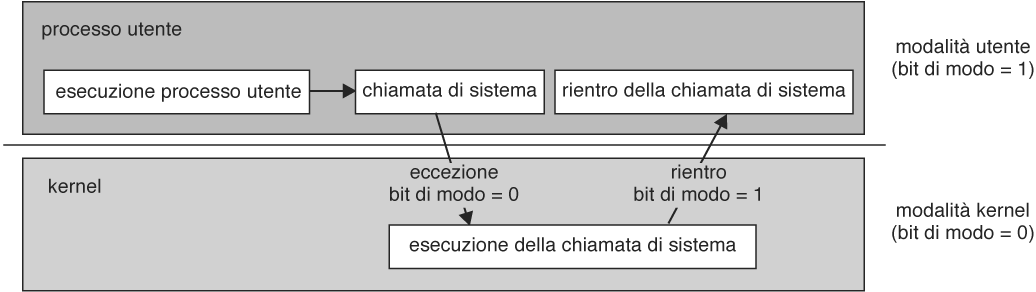
\includegraphics[width=0.5\linewidth]{images/so-process-managing.png}
\end{figure} \\
Si dice di solito che il processo utente sta eseguendo in \textbf{kernel mode}

\subsection{Timer}

\qs{}{
Che succede se un programma utente, una volta ricevuto il controllo dalla CPU, si mette ad eseguire il seguente codice: $for(;;)i++;$?
}
Per evitare questo tipo di problemi, nella CPU è disponibile un \textbf{Timer}, che viene inizializzato con la quantità di tempo che si vuole concedere \textbf{consecutivamente} al programma in esecuzione.\\
Qualsiasi cosa faccia il programma in esecuzione, dopo 1/10 di secondo il Timer invia un \textbf{interrupt} alla CPU, e il controllo viene restituito al sistema operativo.
Il SO \textbf{verifica} che tutto stia procedendo regolarmente, riinizializza il Timer e decide quale programma mandare in esecuzione, questa è l'essenza del \textbf{time-sharing}

\clm{}{}{Ovviamente, le istruzioni macchina che gestiscono il timer, sono istruzioni privilegiate.\\ Altrimenti un programa utente potrebbe modifcare semplicemente i valori :D}

\subsection{Protezione della memoria}
\qs{}{Cosa succede se un programma in esecuzione scrive i dati di un altro programma in "esecuzione"?}
E’ necessario proteggere la memoria primaria da accessi ad aree riservate.

\subsubsection{Due possibili soluzioni}
Una possibile soluzione: in due registri appositi della CPU (base e limite) il SO carica gli indirizzi di inizio e fine dell’area di RAM assegnata ad un programma.\\
Ogni indirizzo I generato dal programma in esecuzione viene \textbf{confrontato} con i valori contenuti nei registri base e limite. \\
$$\text{Se }I < \text{base } || I > \text{limite} \Longrightarrow \text{ TRAP!}$$ \\
I controlli vengono fatti in parallelo a livello hardware, altrimenti richiederebbero troppo tempo. \\\\

Un'altra variante: simile: in due registri appositi della CPU il SO carica rispettivamente l’indirizzo di inizio (base) e la dimensione (offset) dell’area di RAM assegnata ad un programma.
$$\text{Se } I < \text{base } || I > \text{base} + \text{offset} \Longrightarrow \text{ TRAP!}$$

% Leggere sezione 1.7, 1.10, 1.11 (Aggiungere)
